
\chapter{None KB-Specific Network(N-KBSN)}
联合嵌入模型是目前视觉问答的主流架构,因为模型训练的便捷性,并且研究者可以对不同的图像特征的提取方法、不同的文本特征的提取方法、两种模态的不同融合方法组合创新,因此从2015年视觉问答任务出现至今,大量的VQA模型都使用了该架构。此外,由于这些模型便于使用统一的数据集作为衡量标准,因此在VQA任务挑战中,绝大多数的模型都是基于该种架构,也取得了较好的表现,2019年的冠军模型能在VQA2.0数据集下获得总体75\%作用的准确率。

为了实现一个通用的VQA架构,并且利用好联合嵌入模型在回答相对简单的识别类问题的便捷性,本章将沿袭联合嵌入模型的思路,提出None KB-Specific Network(N-KBSN)模型。N-KBSN使用在多目标检测中表现优秀的Faster R-CNN\citing{ren2015faster}作为图像特征提取器,使用能够获得上下文信息的ELMo动态词向量\citing{Peters:2018}表示问题文本,并使用从Transformer中借鉴的多头注意力机制\citing{NIPS2017_7181}进一步强化特征的表征能力,最后通过特征融合预测答案。N-KBSN模型的基础架构如图\ref{N-KBSN}。
\begin{figure}[H]
	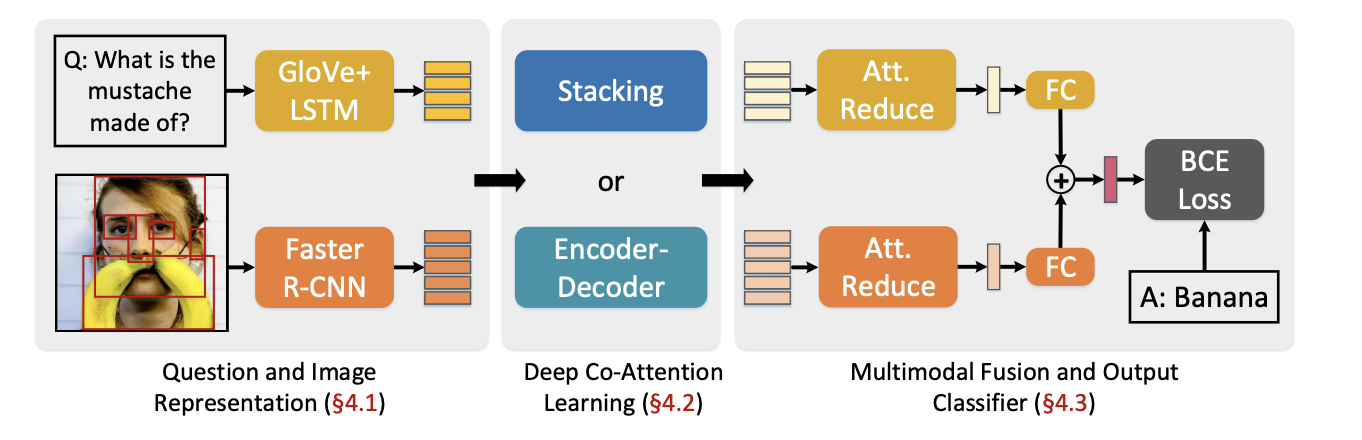
\includegraphics[width=0.8\textwidth]{N-KBSN.png}
	\caption{N-KBSN基本结构}
	\label{N-KBSN}
\end{figure}

\section{基于Faster R-CNN的图像处理}
目标检测是机器视觉领域的重要应用之一,目标检测的核心任务是准确、快速的从图像中定位出目标并且能识别目标的类别、属性等特性。在 2012 年深度学习正式介入计算机视觉目标检测任务之前,传统的目标检测算法一直是以滑动窗口卷积等较为传统的方式进行区域选择、特征提取和分类回归等步骤,例如可变形的组件模型(DPM)方法\citing{felzenszwalb2009object}等。这些传统的目标检测算法大多区域选择的策略效果差、时间复杂度高,并且因为由于是人工提取特征,提取的特征层次较低,致使模型的鲁棒性较差。在深度学习兴起并逐渐成为计算机视觉的核心方法之后,大批优秀的目标检测算法出现,例如R-CNN\citing{girshick2014rich}、SPP-Net\citing{he2015spatial}、Fast R-CNN\citing{girshick2015fast}、Faster R-CNN\citing{ren2015faster}、Mask R-CNN\citing{he2017mask}、YOLO\citing{redmon2016you}及其后续版本等。以上的模型大致分为两个主要类别,第一类为两级式检测框架,包含一个用于区域提议的预处理步骤,使得整体流程是两级式的,例如一系列的R-CNN模型;第二类为单级式检测框架,即无区域提议的框架,这是一种单独提出的方法,不会将检测提议分开,使得整个流程是单级式的,例如YOLO系列的模型。由于Faster R-CNN在各个目标识别任务的出色表现,本节将省略对单级式检测框架的介绍,并着重介绍本文中图像处理的核心模型Faster R-CNN。

区别于传统的滑动卷积窗口来判断目标的可能区域,R-CNN 采用选择性搜索的方法来预先提取一些可能包含目标物体的候选区域(region proposal),再使用卷积神经网络提取各个图像区域的特征,再将提取的特征送入SVM分类器完成类别识别,最后使用回归器对目标位置进行修正。这种方法显著的提升识别速度,降低了计算成本,也提高了准确率。因为R-CNN需要分别对每一个生成的候选区域进行一次特征提取,存在着大量的重复运算,制约了算法性能。为了减少R-CNN的重复计算,研究者提出了SPP-Net。该算法通过在网络的卷积层和全连接层之间加入空间金字塔池化层(Spatial Pyramid Pooling)来对利用 CNN 进行卷积特征提取之前的候选区域进行裁剪和缩放使 CNN 的输入图像尺寸一致。随后的Fast R-CNN借用了SPP-Net的空间金字塔池化层,设计了兴趣区域池化(RoI Pooling),将图像中的多个兴趣区域池化成相同大小的特征图,并使用这些特征图同时预测物体类别和框出对象的区域。这种方法解决了输入候选区域尺寸不一致的问题,并且提高了计算速度。但是Fast R-CNN在生成生成候选区域的较慢,为了解决这一问题,R-CNN的作者又提出了Faster R-CNN。

Faster R-CNN同样沿袭了先前R-CNN和Fast R-CNN的两级式检测框架,但是为了解决之前的大量候选框导致的速度慢的问题,Faster R-CNN设计了一个用于选择和判断候选区域候选网络(Region Proposal Network, RPN),该网络将CNN处理后的全局图像特征作为输入,输出候选区域,最终的分类器结合全局的图像特征和候选区域预测各个区域的类别。
\begin{figure}[H]
	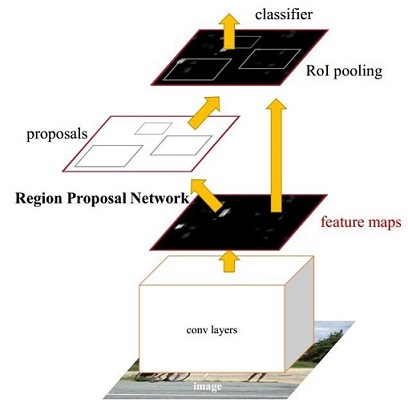
\includegraphics[width=0.5\textwidth]{Faster_R_CNN.png}
	\caption{Faster R-CNN基本结构}
	\label{Faster_R_CNN}
\end{figure}

如图\ref{Faster_R_CNN},Faster R-CNN可以根据功能的不同将模型分为四个模块:卷积层、候选区域候选网络(RPN)、兴趣区域池化(RoI Pooling)、分类器。卷积层使用CNN及其变型提取图像特征,生成的特征图被共享用于后续RPN层和全连接层,这种对图像的处理方式不同于R-CNN和Fast R-CNN。后两者都是先从原始图像中提取候选区域,再分别对候选区域提取特征。RPN网络用于预测候选区域,该网络在CNN输出的图像特征上滑动,在每个空间区域,网络都会预测类别得分,通过softmax判断锚点(anchors)属于前景(foreground)或者背景(background),利用候选框回归(bounding box regression)修正锚点获得精确的候选区域。兴趣区域池化层收集输入的特征图和候选区域,综合这些信息后提取候选区域特征图,送入后续全连接层判定目标类别。分类器利用候选区域特征图计算区域的类别,同时再次使用候选框回归获得检测框最终的精确位置。

在本文中,我们使用联合在ImagNet\citing{russakovsky2015imagenet}上预训练的ResNet-101和在Visual Genome\citing{krishna2017visual}上预训练Faster R-CNN提取图像特征。给定图像$I$,我们从图像中提取$k$个大小不固定的图像特征,$V=\{v_1, v_2, ..., v_k\}, v_i \in \mathbb{R}^D$,每一个图像特征编码一个图像区域。对卷积层输出的特征图,使用非极大抑制(non-maximum suppression)和单元重合(IoU)阈值筛选出排名靠前的候选区域。对于每个所选区域$i$,$v_i$被定义为该区域的特征图的均值池化结果,并将$k$个区域的$v_i$拼接成为最终的图像特征,文本使用的图像特征维度为2048。

\section{基于ELMo的文本处理}
和众多自然语言处理任务一样,在视觉问答任务中如何准确理解问题内容对最终的答案准确率上有着决定性的影响。而自然语言理解中最为基本和核心的便是文本表达,文本表达将自然语言转换为计算机可处理的数字,为自动化处理文本相关的任务建立了基础。在文本表达中,独热向量(one-hot)是最早也是最为简单的词向量。但是其稀疏性会带来的“维度灾难”和因简单的编码方式而造成“语义鸿沟”。基于分布式假设——即处于相似上下文的词语具有相似的含义,研究者先后提出了多种使用分布式表示的词向量模型,例如,CBOW,Skip-Gram,word2vec\citing{mikolov2013distributed},潜在语义分析(LSA)\citing{landauer1998introduction},GloVe\citing{pennington2014glove},ELMo\citing{Peters:2018},BERT\citing{DBLP:journals/corr/abs-1810-04805}等。

CBOW和Skip-Gram均是使用神经网络模型训练上下文信息得到词向量。word2vec也使用了CBOW与Skip-Gram来训练模型与得到词向量,但是并没有使用传统的DNN模型,而是使用霍夫曼树来代替隐藏层和输出层的神经元,提高了计算效率,因此被研究者广泛地使用作为预训练的词向量。但是由于word2vec使用滑动窗口来限定上下文信息,因此得到的词向量仅仅使用了局部的语义和语法信息。不同于word2vec使用局部语料,潜在语义分析(LSA)采用统计计数的方式获得语料的全局信息,其统计预料库中每两个词共同出现的次数构成共现矩阵,并采用了基于奇异值分解(SVD)的矩阵分解技术对大矩阵进行降维,得到词向量。然而LSA方法中的SVD计算量很大,并且共现矩阵仅能表示两个词语同时出现的次数,并不能表示词语之间的远近关系。为了改进word2vec的局部预料限制和LSA的计算复杂性,GloVe使用衰减函数改造LSA的共现矩阵,使得词语间的远近关系得以表达。GloVe还构建了词向量和共现矩阵之间的近似关系,使用梯度下降算法取代了LSA中的奇异值分解,大大减少了计算代价,并且得到了远超LSA和word2vec的性能。

以上提到的所有模型都是通过对语料库的学习得到静态的词向量,即每个单词对应一个确定的实数向量,这种固定向量在处理词汇的多义性上表现不佳。无论是中文词语还是英文单词都广泛得存在一词多义的现象,即同一个词在不同的语境下含义发生变化,例如,在中文中,“他正在算账”和“下回找你算账”中的“算账”由于文化演化而产生了更复杂的引申义,又如英文中的“where is the bank?”和“It is the bank of the river”中的“bank”在第一句中译为“银行”而第二句中译为“河畔”。为解决一词多义的问题,研究者提出了动态词向量,ELMo和BERT便是其中的代表。ELMo在多个NLP任务中均提高了模型的准确率,因此本文将着重介绍并使用ELMo模型处理视觉问答任务中的文本,并在后续的处理中结合类似于BERT的注意力机制。

ELMo是一种深度场景化的词表示。其模型深度能够对复杂的词语使用特性——语法和语义特征进行有效建模,而其模型的动态性能根据词语的上下文的不同生成动态向量,进而为解决一词多义提供了可能。ELMo采用了两个阶段获得词向量,第一个阶段是用大量的文本语料训练一个深度双向语言模型(biLSTM);第二个阶段从预训练网络中提取对应单词的网络各层的内部状态(internal state),并通过函数转化为词向量。

语言模型是对语句的概率分布的建模。语言模型分为前向和后向,前向是指已知上文的词语,推理下一个词语的方式,而后向则是已知后文的内容,求解上一个词语的方式。对于一个具有N个单词的句子$S=(t_1, t_2, ..., t_N)$而言,前向语言模型就是求解以下公式的最大值:
\begin{equation}
p(t_1, t_2, ..., t_N)=\prod_{k=1}^N p(t_k|t_1,t_2,...,t_{k-1})
\end{equation}
其中$p(t_1, t_2, ..., t_N)$为序列的联合概率,
$p(t_k|t_1, t_2,..., t_{k-1})$表示已知$t_k$的上文$(t_1, t_2, ..., t_{k-1})$的条件下,求解$t_k$的条件概率。对应的后向语言模型的公式为
\begin{equation}
p(t_1, t_2, ..., t_N)=\prod_{k=1}^N p(t_k|t_{k+1},t_{k+2},...,t_N)
\end{equation}

ELMo使用双向LSTM(biLSTM)模型作为语言模型的基础。首先将“上下文无关的”初始词向量$x{_k^{LM}}$输入L层的前向LSTM。在位置k上,LSTM将输出一个“上下文相关”的词表征$\vec{h}_{k,j}^{LM,j}$,其中$j = 1, ..., L$。最后一层的LSTM输出$\vec{h}_{k,j}^{LM,L}$通过一个softmax层预测下一个词语的初始词向量$x{_{k+1}^{LM}}$。后向LSTM类似于前向LSTM有L层并且在k位置上得到一个词表征$\overleftarrow{h}_{k,j}^{LM}$。最后通过最大似然的方式训练双向LSTM模型,公式如下:
\begin{equation}
\sum_{k=1}^N(\log_p(t_k|t_1, t_2,..., t_{k-1};\Theta_x,\overrightarrow{\Theta_{LSTM}},\Theta_s) + \log_p(t_k|t_{k+1},t_{k+2},...,t_N;\Theta_x,\overleftarrow{\Theta_{LSTM}},\Theta_s)
)
\end{equation}

其中,$\Theta_x$和$\Theta_s$分别是初始词向量训练时的两个softmax层参数,$\overrightarrow{\Theta_{LSTM}}$和$\overleftarrow{\Theta_{LSTM}}$则是双向语言模型的参数。

当完成预训练阶段后,向网络输入一个新句子,句子中每个单词都能得到对应的三种Embedding:最底层是初始的词向量$x{_k^{LM}}$;前向LSTM输出的$\overrightarrow{h}_{k,j}^{LM}$;后向LSTM输出的$\overleftarrow{h}_{k,j}^{LM}$。ELMo将三种词向量串联,得到
\begin{equation}
R_k = 
[x_k^{LM}, \overrightarrow{h}_{k,j}^{LM}, \overleftarrow{h}_{k,j}^{LM} | j = 1, ..., L]
= [h_{k,j}^{LM} | j = 0, ..., L]
\end{equation}

其中$h_{k,0}^{LM}$是初始词向量,$h_{k,j}^{LM} = [\overrightarrow{h}_{k,j}^{LM}; \overleftarrow{h}_{k,j}^{LM}]$ 是每个biLSTM层输出的结果。

最后使用以下公式得到对应单词的具有”上下文信息“的词向量。
\begin{equation}
ELMo_k^{task} = E(R_k; \Theta^{task}) = \gamma^{task}\sum_{j=0}^L s_j^{task} h_{k,j}^{LM}
\end{equation}

其中是$s_j^{task}$任务相关训练得到的权重参数, $\gamma$是一个任务相关的scale参数。

在本文中,我们将问题文本分割为单词组成的列表,并将每个单词转化为50维的初始词向量,即$x_k^{LM}\in \mathbb{R}^{50}$,设定双向语言模型的层数$L = 2$,隐层节点数$H_{dim} = 4096$,输出维度$output_{dim} = 512$,因此$ELMo_k^{task}$维度为1024。

\section{自注意力(SA)与引导注意力(GA)}
正如绪论中提到的,注意力机制的引入帮助神经网络提高了预测精度,并且减少了计算复杂度。视觉问答任务由于需要处理多模态的数据——图像和文本,比起仅需要处理单模态的数据的任务更需要进行高效的计算。同时,VQA任务输入的图像和问题文本具有高度的相关性,因此两种模态的数据之间的交互对于结果的准确性的提升也具有显著的影响。对于以上两个需求,我们在N-KBSN中使用了Transformer\citing{NIPS2017_7181}的多头注意力机制(Multi-head Attention, MA)实现图片的自注意力(V-SA)、问题文本的自注意力(Q-SA)、由问题引导的对图像的注意力(Guided Attention, GA)。

注意力机制本质上是找到一个方式对已有信息分配合适的权重,并以此提高输出的准确性。我们可以将注意力函数描述成映射查询(query)到一些键值对(key-value pair)并由此得到输出。假定查询矩阵$Q = \{q_1, q_2, ..., q_m\}$,其中查询向量$q_i \in \mathbb{R}^{1 \times d_q}$;key矩阵$K = \{k_1, k_2, ..., k_n\}$,其中$k_j\in \mathbb{R}^{1 \times d_k}$;value矩阵$V = \{v_1, v_2, ..., v_n\}$,其中value向量$v_i \in \mathbb{R}^{1 \times d_v}$,那么注意力特征可以通过对value矩阵的加权得到,权重可以通过查询矩阵和key矩阵得到:
\begin{equation}
Attention(Q, K, V) = score(Q, K)V
\end{equation}
其中$score(Q, K)$为计算权重的函数,有多种计算方式,本文使用Transformer中的缩放点乘法:
\begin{equation}
score(Q, K) = softmax(\frac{QK^T}{\sqrt{d_k}})
\end{equation}
其中$q_i$和$k_j$要求具有相同的维度。
因此可以得到:
\begin{equation}
Attention(Q, K, V) = softmax(\frac{QK^T}{\sqrt{d_k}})V
\end{equation}

为了进一步提高注意力特征的表达能力,引入多头注意力机制。多头注意力机制的实现过程是,将上式的$Q, K, V$输入到$h$个具有不同权重的线性层,得到$(Q_i, K_i, V_i), i = 1, 2, ..., h$,再分别计算得到$Attention(Q_i, K_i, V_i), i = 1, 2, ..., h$,最后将$h$个注意力特征拼接并通过一个线性层获得期望维度的注意力特征,如图\ref{ma}。多头注意力机制的公式为:
\begin{equation}
MA(Q, K, V) = [head_1, head_2, ..., head_h]W
\end{equation}
\begin{equation}
head_i = Attention(Q_i, K_i, V_i)
\end{equation}
其中$W$为线性层的权重。
\begin{figure}[H]
	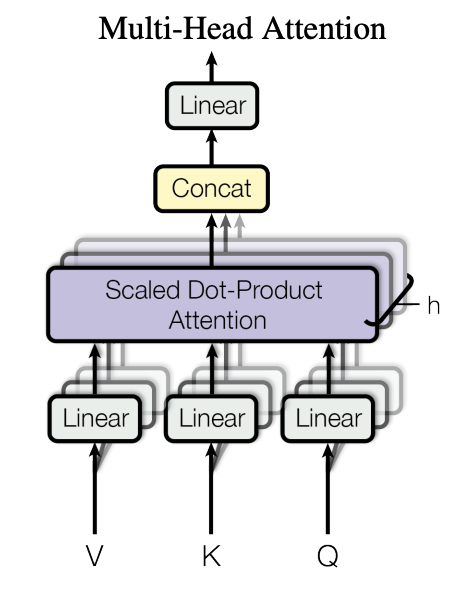
\includegraphics[width=0.5\textwidth]{ma.png}
	\caption{多头注意力的架构。多头注意力特征由h个缩放点乘注意力特征拼接得到。}
	\label{ma}
\end{figure}

基于以上多头注意力机制的思想,本文分别使用三种注意力特征:图片的自注意力(V-SA)、问题文本的自注意力(Q-SA)、由问题引导的对图像的注意力(GA)。假设文本词向量矩阵为$Y$,图像特征图为$X$,则在计算V-SA时,$Q = K = V = X$,在计算Q-SA时,$Q = K = V = Y$;在计算引导注意力特征时,$Q = Y$为词向量矩阵,$K = V = X$为图像特征矩阵,并且词向量和图像特征向量具有相同的维度。三种注意力组合的结构构成一个共同注意力模块(MCA),结构如图\ref{mca}。
\begin{figure}[H]
	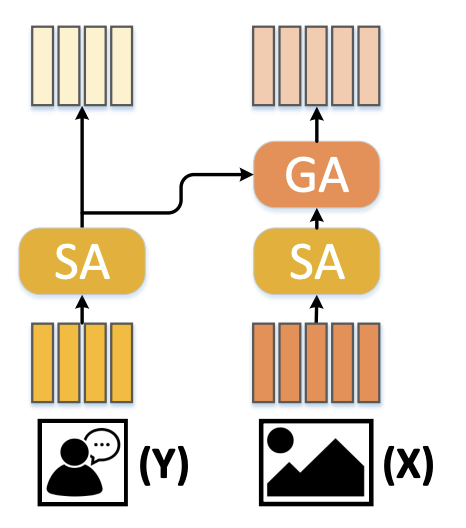
\includegraphics[width=0.3\textwidth]{mca.png}
	\caption{共同注意力模块(MCA)由一个V-SA、一个Q-SA和一个GA组成。}
	\label{mca}
\end{figure}

为了提高使用深度的注意力机制提取更高层次的特征,MCAN论文\citing{Yu_2019_CVPR}提出了Encoder-Decoder和Stacking两种级联MCA层的方式,如图\ref{mca_stacking}。
\begin{figure}[H]
	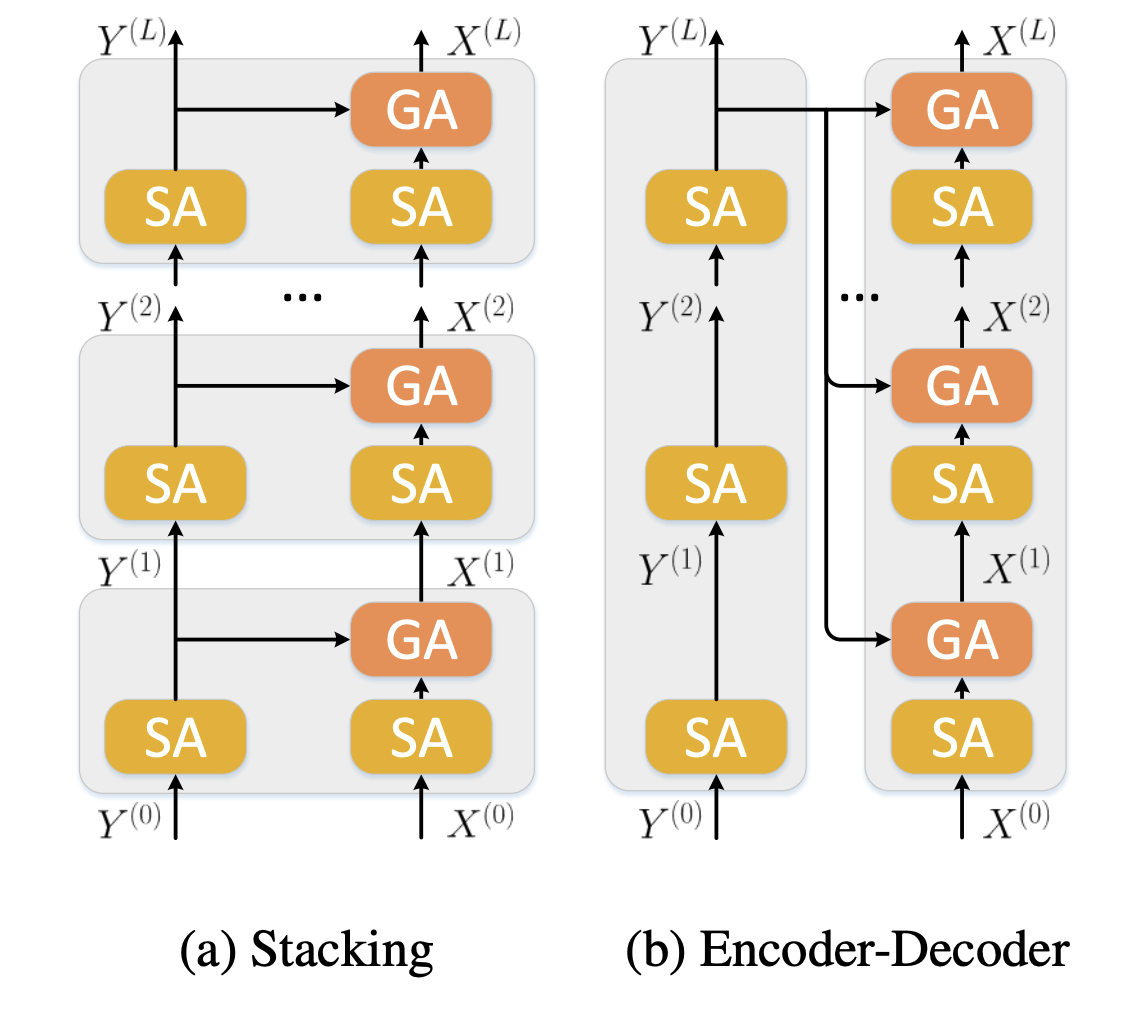
\includegraphics[width=0.5\textwidth]{mca_stacking.png}
	\caption{两种MCA层的级联方式,Stacking将上一层的输出直接作为下一层的输入,Encoder-Decoder将最后一层的问题自注意力特征作为每一层图像的查询矩阵。}
	\label{mca_stacking}
\end{figure}

根据文章给出的两种级联方式在多个任务的表现情况\citing{Yu_2019_CVPR},在本文中,我们使用Stacking的级联方式,并将设置不同的层数$L$,探究不同深度下注意力机制对模型的影响。

\section{实验}
\subsection{超参数配置}
\subsection{剔除研究}
\subsection{实验结果分析}

\section{结论}
